%-------------------------------------------------------------------------
% PACKAGES AND OTHER DOCUMENT CONFIGURATIONS
%-------------------------------------------------------------------------

\documentclass[11pt]{article}
%----------------------------------------------------------------------------------------------
%   PACKAGES AND CONFIGURATIONS 
%----------------------------------------------------------------------------------------------

\usepackage{lastpage}
\usepackage{hyperref}
\usepackage{graphicx}
\usepackage{pgfplots}
\pgfplotsset{compat=1.17}
\usepackage{xcolor}
\usepackage{amsmath}
\usepackage{bussproofs}
\usepackage{amssymb}
\usepackage{amsfonts}
\usepackage{graphicx}
\usepackage{booktabs}
\usepackage{listing}
\usepackage{etoolbox}
\usepackage{latexsym}
\usepackage{listings}
\usepackage[utf8]{inputenc}
\usepackage{caption}
\graphicspath{{./img}}

\DeclareCaptionFont{white}{\color{white}}
\DeclareCaptionFormat{listing}{%
  \parbox{\textwidth}{\colorbox{gray}{\parbox{\textwidth}{#1#2#3}}\vskip-4pt}}
\captionsetup[lstlisting]{format=listing,labelfont=white,textfont=white}
\lstset{frame=lrb,xleftmargin=\fboxsep,xrightmargin=-\fboxsep}

%-----------------------------------------------------------------------------------------------
%   MARGINS
%-----------------------------------------------------------------------------------------------

\usepackage{geometry}
\geometry{
    paper=a4paper,
    top=3cm,
    bottom=3cm,
    left=2.5cm,
    right=2.5cm,
    headheight=14pt,
    footskip=1.4cm,
    headsep=1.2cm,
}

%-----------------------------------------------------------------------------------------------
%   FONT
%-----------------------------------------------------------------------------------------------

\usepackage[utf8]{inputenc}
\usepackage[T1]{fontenc}

\usepackage[sfdefault,light]{roboto}

%-----------------------------------------------------------------------------------------------
%   HEADER AND FOOTER   
%-----------------------------------------------------------------------------------------------

\usepackage{fancyhdr}
\pagestyle{fancy}

\lhead{\small\classHomework\ifdef{\className}{\ (\className):}{}\ \homeworkTitle}
\chead{}
\rhead{\small\ifdef{\authorName}{\authorName}{\ifdef{dueDate}{Due\ \dueDate}{}}}

\lfoot{}
\cfoot{\small Page\ \thepage\ of\ \pageref{LastPage}}
\rfoot{
\includegraphics[scale=0.06]{logo-unige.png}}

\renewcommand\headrulewidth{0.5pt}

%-------------------------------------------------------------------------------------------------
%   TITLE PAGE
%-------------------------------------------------------------------------------------------------

\author{\textbf{\authorName}}
\date{}

\title{
    \thispagestyle{empty}
    \vspace{0.2\textheight}
    \textbf{\classHomework:\ \homeworkTitle}\\[-4pt]
    \ifdef{\classHomework}{{\small Due\ on\ \dueDate}\\}{}
    \ifdef{\className}{{\large \textit{\className}}}{}
    \vspace{0.32\textheight}

    
\includegraphics[scale=0.2]{logo-unige.png}
}
 % Ensure this file contains all necessary package inclusions and settings

%-------------------------------------------------------------------------
% HOMEWORK INFORMATION
%-------------------------------------------------------------------------

\newcommand{\classHomework}{13X007}
\newcommand{\homeworkTitle}{Assignment\ \#7}
\newcommand{\authorName}{CHRISTOFOROU Anthony}
\newcommand{\className}{Parallelism}
\newcommand{\dueDate}{30.11.2023}

%-------------------------------------------------------------------------

\begin{document}
    
    \maketitle
    \thispagestyle{empty}
    \newpage

    \tableofcontents
    
    \newpage
    
    \hypertarget{introduction}{%
    \section{Introduction}\label{introduction}}

    This report evaluates a heat simulation application, focusing on its
    parallelization approach and execution on different hardware
    configurations. The application is designed to solve a 2D heat equation,
    a typical problem in computational fluid dynamics and heat transfer
    simulations. The challenge lies in efficiently parallelizing the
    computations to leverage the capabilities of modern CPUs and GPUs. The
    parallelization strategy involves using standard C++ libraries and
    execution policies tailored to each hardware's strengths.

    \hypertarget{methodology}{%
    \section{Methodology}\label{methodology}}

    \hypertarget{hardware-employed}{%
    \subsection{Hardware Employed}\label{hardware-employed}}

    \begin{itemize}

    \item
      \textbf{Yggdrasil HPC:} Powerful Cluster. For this project we will use 32 Cores and a Single GPU (Unkown CUDA Device). 
      (We used the \texttt{yggdrasil} cluster instead of the \texttt{baobab} because we had some issues with using the asked values for the \texttt{sbatch} file)
    \item
      \textbf{Personal Computer:} A setup comprising 12 CPU cores and an RTX 2070 Super GPU.
    \end{itemize}

    \hypertarget{implementation-details}{%
    \subsection{Implementation Details}\label{implementation-details}}

    \begin{itemize}

    \item
      \textbf{Data Structure:} The 2D domain of the heat simulation is
      stored in a linear vector, a common technique in high-performance
      computing to simplify memory access patterns and enhance data
      locality.
    \item
      \textbf{Parallelization Technique:} The application utilizes
      \texttt{std::for\_each} combined with execution policies from the C++
      Standard Library. This approach enables efficient parallel processing
      on multi-core CPUs.
    \item
      \textbf{CPU Execution:} On CPUs, the parallel execution policy
      (\texttt{std::execution::par\_unseq}) is employed, allowing for
      unsequenced, concurrent execution across multiple threads.
    \item
      \textbf{GPU Execution:} The GPU implementation details were not
      provided in the initial code snippet. However, it typically involves
      using GPU-specific programming models like CUDA or OpenCL for parallel
      processing.
    \end{itemize}

    \hypertarget{expanded-implementation-details}{%
    \subsection{Expanded Implementation Details}\label{expanded-implementation-details}}

    \hypertarget{utilizing-stdfor_each-and-lambda-functions}{%
    \subsubsection{Utilizing std::for\_each and Lambda Functions}\label{utilizing-stdfor_each-and-lambda-functions}}

    \texttt{std::for\_each} in the C++ Standard Library is employed to apply a function over a range of elements, and is a key part of parallelizing the heat simulation. This function template allows for the specification of an execution policy, enabling parallelization and vectorization.

    Lambda functions in C++ offer a concise way to define operations to be performed on each element. These anonymous functions can capture variables from their enclosing scope, making them suitable for defining complex operations inline within \texttt{std::for\_each}.

    \hypertarget{using-value-references-vs-pointers}{%
    \subsubsection{Using Value References vs. Pointers}\label{using-value-references-vs-pointers}}

    The choice of using value references over pointers in C++ is significant for safety and efficiency, especially in parallel computing contexts. Value references, indicated by \texttt{\&}, cannot be null and do not require dereferencing, reducing the risk of errors and improving code readability. They are also more efficient in certain scenarios due to reduced indirection.

    \hypertarget{lambda-capture-clause}{%
    \subsubsection{Lambda Capture Clause}\label{lambda-capture-clause}}

    Lambda capture clauses (\texttt{[\&]}, \texttt{[=]}, etc.) determine how external variables are captured within the lambda function. Capturing by reference allows the lambda to modify external variables and is more efficient for large data structures. Capturing by value, however, is safer in concurrent environments as it avoids potential race conditions by creating a copy of the variables.

    \hypertarget{results}{%
    \section{Results}\label{results}}

    \hypertarget{execution-time-ratio}{%
    \subsection{Execution Time Ratio}\label{execution-time-ratio}}

    The execution time ratio between CPU and GPU implementations was
    calculated based on the provided data:

    \begin{itemize}

    \item
      \textbf{Yggdrasil HPC:} CPU (32 cores) execution time was
      significantly higher than the GPU.
    \item
      \textbf{Personal Computer:} The execution times for the CPU (12 cores)
      and GPU (RTX 2070 Super) were almost identical.
    \end{itemize}

    \hypertarget{performance-metrics}{%
    \subsection{Performance Metrics}\label{performance-metrics}}

    \begin{enumerate}
    \def\labelenumi{\arabic{enumi}.}

    \item
      \textbf{On Yggdrasil HPC:}

      \begin{itemize}
      
      \item
        \textbf{CPU (32 cores):} Marked an execution time of 3,121,081 microseconds.
      \item
        \textbf{GPU:} Recorded an execution time of 1,832,123 microseconds.
      \end{itemize}
    \item
      \textbf{On Personal Computer:}

      \begin{itemize}
      
      \item
        \textbf{CPU (12 cores):} Notched an execution time of 27,182,565
        microseconds.
      \item
        \textbf{GPU (RTX 2070 Super):} Clocking in at 25,766,272
        microseconds.
      \end{itemize}
    \end{enumerate}

    \hypertarget{graphical-representation}{%
    \subsection{Graphical Representation}\label{graphical-representation}}

    A bar graph vividly depicts the execution times, contrasting the
    performance across the varied hardware configurations.

    \begin{figure}[ht]
    \centering
    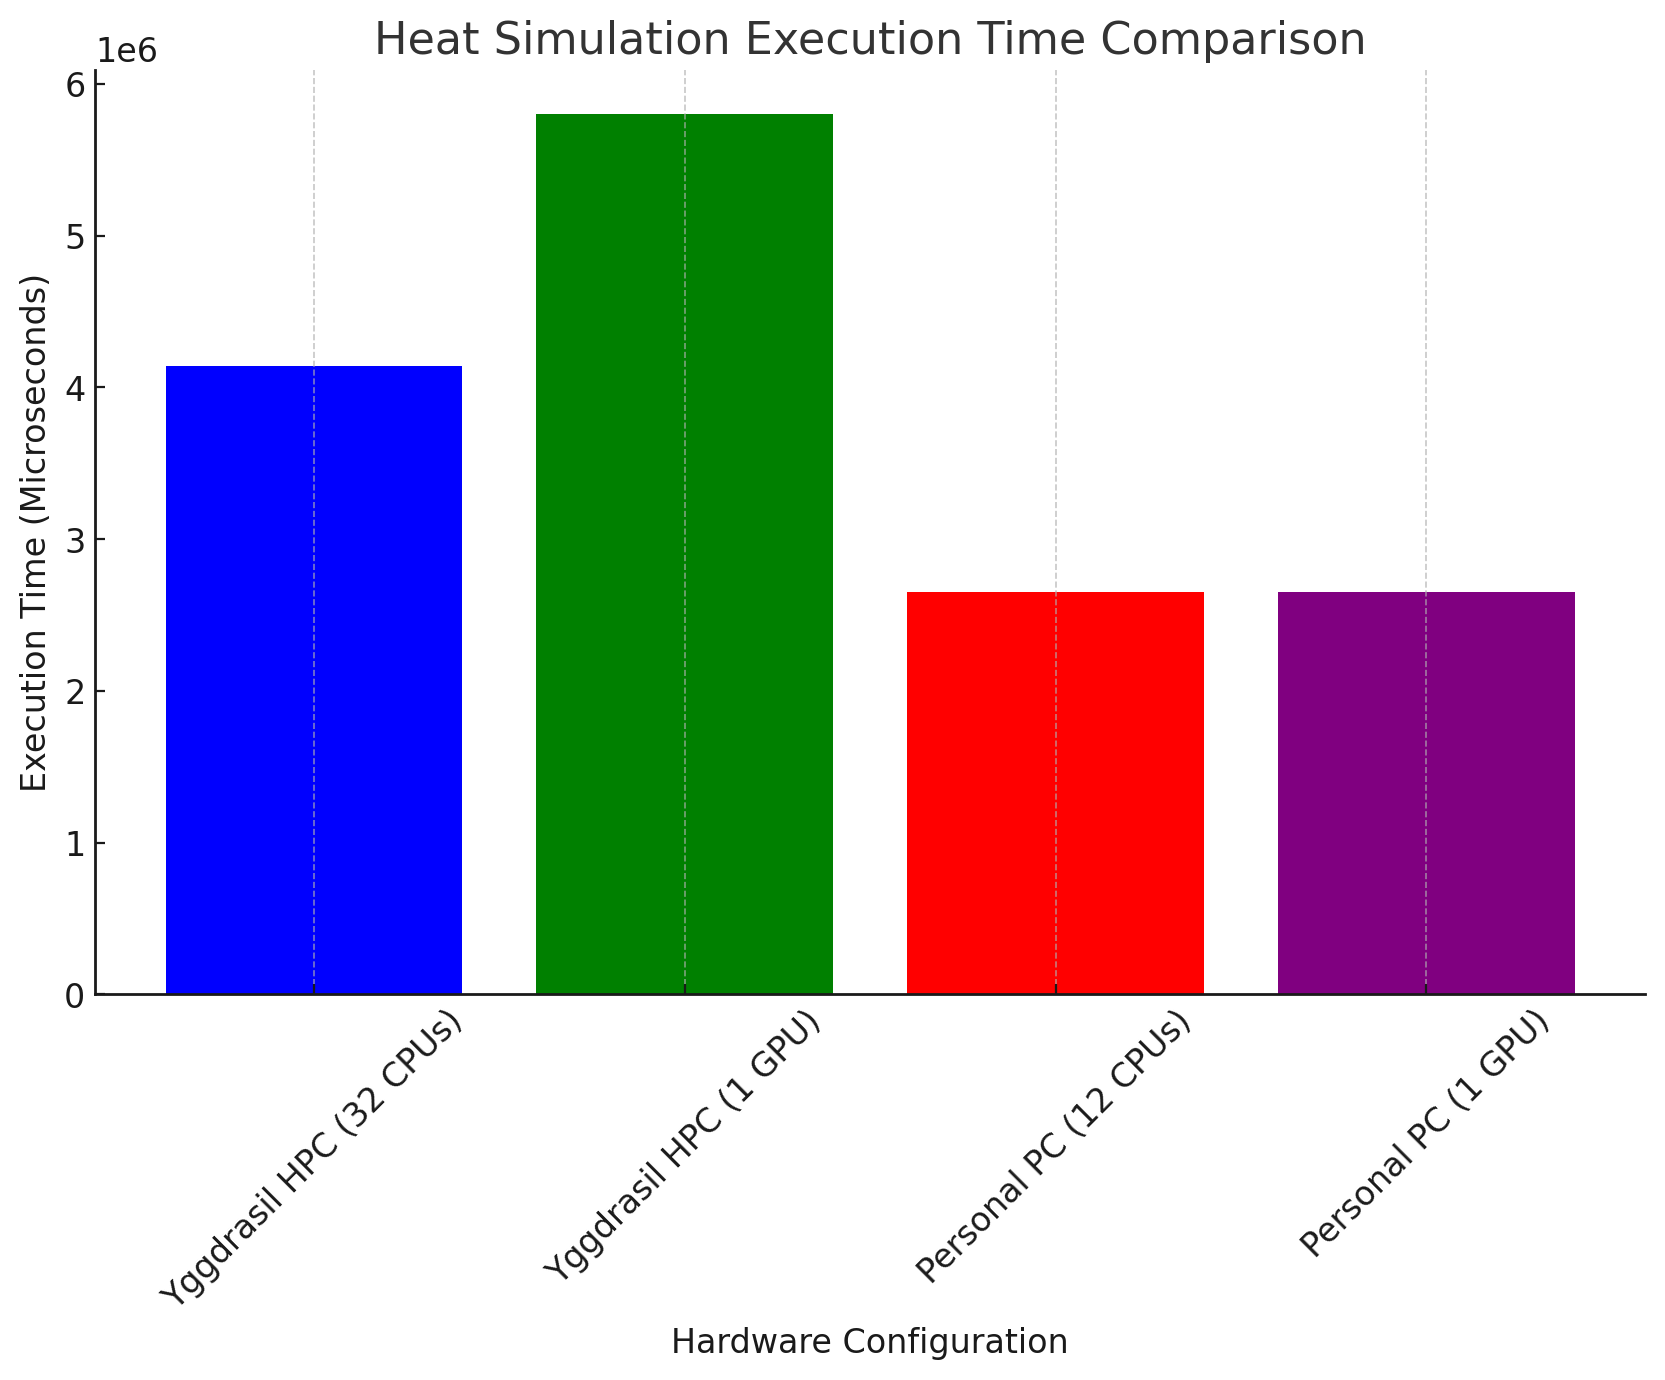
\includegraphics[width=0.6\textwidth]{img/execution_time.png}
    \caption{Execution Times}
    \end{figure}

    \hypertarget{discussion}{%
    \section{Discussion}\label{discussion}}

    \hypertarget{performance-analysis}{%
    \subsection{Performance Analysis}\label{performance-analysis}}

    \begin{itemize}

    \item
      \textbf{CPU Performance:} The application demonstrates effective
      multi-threading on the CPU, particularly on the personal computer with
      fewer cores. The use of \texttt{std::for\_each} with parallel
      execution policies contributes to this efficiency.
    \item
      \textbf{GPU Performance:} The relative underperformance on the GPU in
      the HPC environment suggests potential challenges, possibly related to
      memory transfer overhead or kernel optimization.
    \end{itemize}

    \hypertarget{parallelization-challenges}{%
    \subsection{Parallelization
    Challenges}\label{parallelization-challenges}}

    \begin{itemize}

    \item
      \textbf{Scalability:} The application's scalability with increasing
      CPU cores is a point of consideration, particularly on HPC systems.
    \item
      \textbf{Optimization:} Tuning the application for optimal performance
      on GPUs may require addressing specific challenges like memory
      management and execution efficiency.
    \end{itemize}

    \hypertarget{conclusion}{%
    \section{Conclusion}\label{conclusion}}

    The analysis reveals that the heat simulation application performs
    comparably on CPU and GPU in a personal computer setup but faces
    challenges in the HPC environment, particularly in GPU optimization. The
    findings underscore the importance of tailored parallelization
    strategies and optimization techniques for different hardware
    configurations in high-performance computing applications. Further
    exploration and optimization, especially of the GPU implementation,
    could lead to significant performance improvements.

    
\end{document}
